\chapter{Game Engines}\label{ch:gameengines}
In diesem Kapitel soll die Theorie und Algorithmen aus den vorherigen Kapiteln 
getestet werden. Manche Game Engines bieten auch eigene Speichersysteme oder
Tools dafür, diese können hier auch getestet werden.

Gleiche Szene in verschiedenen Game Engines testen. 
Verschiedene Speichersysteme ausprobieren und wenn vorhanden über die von den Game Engines erzählen und ausprobieren.

Zu testende Game Engines: Unity, Unreal Engine, Godot

Szene zum testen soll sehr viele Daten zu speichern haben (Große Map und viele unterschiedliche Informationen)
%--------------------------------------------------------------------------


%--------------------------------------------------------------------------
\section{Unity}
Unity Engine grob vorstellen und erklären

% 10.7.
\url{https://blog.unity.com/games/persistent-data-how-to-save-your-game-states-and-settings}


\subsection{PlayerPrefs}
Bei Speicher- und Ladesystemen bietet Unity für Entwickler wenige eingebaute Funktionen. Einer der wenigen Funktionen, die Unity bereitstellt sind die PlayerPrefs. Sie eine einfache Art Daten zu speichern, aber ist dabei auch sehr limitiert. Die PlayerPrefs Klasse besitzt wenige Funktionen, denn es werden nur die Datentypen string, float und integer unterstützt. Über einen Schlüssel lässt sich dann ein Schlüsselwert dieser Datentyppen festlegen oder es kann dieser erhalten werden. Die Werte der PlayerPrefs Klasse werden mit der klasseninternen Save-Funktion gespeichert. Diese kann während der Laufzeit im Code aufgerufen werden und wird automatisch bei der Terminierung des Spieles aufgerufen.\cite{unityPlayerPrefsSave} Je nach Betriebssystem werden die PlayerPrefs in einem unterschiedlichen Datei-Format abgespeichert, die Daten werden aber nicht verschlüsselt.
\cite{unityPlayerPrefs}

Allgemein wird davon abgeraten, Unitys PlayerPrefs System für das Speichern des Spielstandes zu verwenden. Zum einen wird für ein Spiel eine Speicherdatei erstellt. Wenn es aber in dem Spiel verschiedene Spielstände geben soll, gibt es bereits Probleme mit diesem Ansatz. Eine mögliche Lösung von diesem Problem wäre es, dass jeder Spielstand eine Identifikationsnummer bekommt, welche dann an jedem Schlüssel hinzugefügt wird. Die ganzen Identifikationsnummern müssen aber auch gespeichert werden, wo auch schon das nächste Problem mit PlayerPrefs auftritt. Es gibt wenige verfügbare Datentypen, die verwendet werden können. Wenn zum Beispiel eine Liste der Identifikationsnummern aller Spielstände gespeichert werden soll, kann dies nicht so einfach gemacht werden. Über den string-Datentyp lassen sich jedoch JSON-Strings speichern, wodurch wieder mehr Datentypen, wie Listen und andere Gruppierungen von Daten, möglich sind. Und PlayerPrefs, was für Player Preferences steht, ist eigentlich auch genaufür die Arten von Daten gemacht. Es sollten Konfigurationen, wie die Auflösung oder die Lautstärke des Spieles, gespeichert werden. Da die Daten auch alle in einer Datei gespeichert werden, ist es auch nicht sonderlich effizient mit vielen Daten zu arbeiten. Effizienter wäre es die Daten auf verschiedene Dateien aufzuteilen, um schnellere Ladezeiten zu erreichen.
\cite{logrocketPlayerPrefs}\cite{gamedevbeginnerPlayerPrefs}

\subsection{JSON}
Die verbreiteste Art mit Unity Spielstände abzuspeichern ist mit JSON. Ein Grund dafür ist, dass Unity ein Tool für das Serialisieren von C\# Objekten hat. Dieses Tool heißt \textit{JsonUtility}, welches über Data Binding die Daten verarbeitet. JsonUtility hat zwar einige Einschränkungen, ist dafür aber die schnellste Art, Objekte in JSON zu serialisieren. Eine Einschränkung von JsonUtility ist, dass es einige Typen gibt, die nicht unterstützt werden, wie Dictionary<>, multidimensionale oder Jagged\footnote{Jagged Arrays sind Arrays, dessen Elemente Arrays aus verschiedener Größe sind.\cite{microsoftVerzweigteArrays}} Arrays. Diese lassen sich nicht mit JsonUtility serialisieren. In dem Beispielcode \ref{lst:jsonUtilityExp} werden die drei Funktionen, die JsonUtility anbietet, demonstriert. Von der Zeile 1 bis 7 wird eine Spieler-Klasse definiert, welche dann in einer anderen Klasse, wie ab der Zeile 11 zu sehen ist, verwendet wird. Diese muss mit dem Attribut "Serializable" gekenntzeichnet werden, damit diese auch serialisierbar ist. Alle Variablen, die in dieser Klasse public oder mit "[SerializeField]" gekenntzeichnet werden, werden beim Serialisierungsprozess betrachtet. Als erstes werden drei Spieler-Objekte definiert, welche in den Zeilen 15 bis 18 zu JSON-Strings serialisiert werden. In der Zeile 16 ist zu sehen, wie einer der JSON-Strings aussieht. Der Spieler mit dem Namen "Bob" wird dann in den letzten zwei Zeilen zwei mal überschrieben. Einmal mit den Werten der Spielerin "Alice" und einmal mit den Werten des Spielers "Tom". 
\cite{unityJsonUtility}\cite{unitySerializationRules} 
\begin{listing}[htp]
    \begin{minted}{csharp} 
        [Serializable]
        public class Player
        {
            public int level;
            public float health;
            public string name;
        }

        ...
        
        Player bob = new Player() { level = 1, health = 75.2f, name = "Bob" };
        Player alice = new Player() { level = 3, health = 100.0f, name = "Alice" };
        Player tom = new Player() { level = 2, health = 1.0f, name = "Tom" };

        string bobJson = JsonUtility.ToJson(bob);
        //  {"level":1,"health":75.2,"name":"Bob"}
        string aliceJson = JsonUtility.ToJson(alice);
        string tomJson = JsonUtility.ToJson(tom);

        bob = JsonUtility.FromJson<Player>(aliceJson);
        JsonUtility.FromJsonOverwrite(tomJson, bob);
    \end{minted}
    \caption{JsonUtility Beispielcode}
    \label{lst:jsonUtilityExp}
\end{listing}

Json.NET:
\begin{itemize}
    \item JSON Serialisierer um Umwandeln zwischen .NET-Objekten zu JSON zu ermöglichen 
    \item Typen die JsonUtility nicht unterstützt gehen hier
    \item Serialisiert alle public Attribute
    \item "[JsonIgnore]" um beim Serialisierer Attribute zu ignorieren
\end{itemize}

% 10.7.
\url{https://www.newtonsoft.com/json}\\
\url{https://www.newtonsoft.com/json/help/html/Performance.htm}\\

LitJSON:\\
% 10.7.
\url{https://litjson.net/}

\url{https://www.jacksondunstan.com/articles/3303}\\
\url{https://michaelscodingspot.com/the-battle-of-c-to-json-serializers-in-net-core-3/}

\begin{figure}[htp]
    \centering
    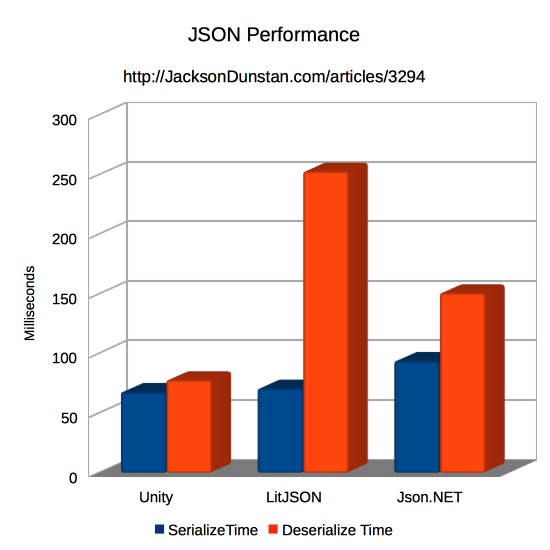
\includegraphics[width=0.6\textwidth]{images/UnityJsonPerformance.png}
    \caption{Laufzeiten der unterschiedlichen JSON Serialisierer für Unity \cite{jacksondunstanJacksonDunstancomJSON}}
    \label{fig:unityJsonPerformance}
\end{figure}

\subsection{BinaryFormatter}
Kurz erwähnen was BinaryFormatter macht und warum er nicht benutzt werden soll. Vielleicht mit einem Beispiel

\begin{itemize}
    \item Serialisieren von Objekten in ein langes stream im binären Format
    \item Serialize(File filename, Object object)
    \item Deserialize(File filename)
    \item Sicherheitsrisiken beim Deserialisieren:
    \begin{itemize}
        \item Angreifer kann ein Denial of Serivce (DoS), Veröffentlichung von Informationen oder Remoteausführung von Code in Ziel-App bewirken
        \item Deserialisieren von Daten mit BinaryFormatter bringt viele Risiken
        \item Angreifer kann Code im Kontext des Zielprozesses ausführen
    \end{itemize}
    \item Sicherere Alternative: BinaryReader und BinaryWriter
    \begin{itemize}
        \item Schreiben/Lesen von primitven Datentypen im binären Format
    \end{itemize}
\end{itemize}

% 10.7.
\url{https://learn.microsoft.com/en-us/dotnet/api/system.runtime.serialization.formatters.binary.binaryformatter?view=net-7.0}\\
\url{https://learn.microsoft.com/en-us/dotnet/standard/serialization/binaryformatter-security-guide}\\
\url{https://github.com/pwntester/ysoserial.net}

\subsection{StreamWriter}
\begin{itemize}
    \item Direktes Schreiben von Zeilen auf Dateien 
    \item Zum Lesen der Zeilen StreamReader
    \item Eignes Format zum Speichern der Klassen bestimmen
    \item Wenn Format geändert wird, kann es schwierig werden Dateien mit altem Format zu verwenden
\end{itemize}

% 10.7.
\url{https://learn.microsoft.com/en-us/dotnet/api/system.io.streamwriter?view=net-7.0}

\subsection{Easy Save}

\begin{itemize}
    \item Unity Package, welches ein komplettes Speicher und Serialisier System ist
    \item ES3.Save(String key, Object value)
    \item ES3.Load<T>(String key, Object defaultValue)
    \item Klassenattribute werden gespeichert, wenn:
    \begin{itemize}
        \item public oder [SerializeField] Attribut haben
        \item Nicht const oder readonly
        \item Nicht [Obsolete] oder [NonSerialized] Attribut
        \item Verschlüsselung mit ES3Settings(ES3.EncryptionType encryptionType, String password)
        \item Komprimierung mit ES3Settings(ES3.CompressionType compressionType)
        \item Auto Save Funktion
    \end{itemize}
\end{itemize}
% 10.7.
\url{https://docs.moodkie.com/product/easy-save-3/}\\
\url{https://assetstore.unity.com/packages/tools/utilities/easy-save-the-complete-save-data-serializer-system-768}

\subsection{Component-Save-System}

\url{https://github.com/AlexMeesters/Component-Save-System}
%--------------------------------------------------------------------------


%--------------------------------------------------------------------------
\section{Unreal Engine}
Unreal Engine grob vorstellen und erklären

\subsection{SaveGame Objekt}
Erklären was das ist, was benutzt wird und ein kleines Beispiel zeigen.

\begin{itemize}
    \item Blueprint zum Speichern/Laden der Daten
    \item Daten in .sav-Datei gespeichert (darüber recherchieren, was das ist und wie Daten hier gespeichert werden. Vor und Nachteile vielleicht auch nennen)
    \item Asynchrones/Syncrhones Speichern/Laden (bei großen Mengen von Daten ist asynchron besser)
\end{itemize}

% 10.7.
\url{https://docs.unrealengine.com/4.27/en-US/InteractiveExperiences/SaveGame/}\\
\url{https://www.tomlooman.com/unreal-engine-cpp-save-system/}

\subsection{JSON}

\begin{itemize}
    \item FJsonSerializer::Serialize((TSharedPtr<FJsonObject> object).ToSharedRef(), TJsonWriterFactory<>::Create(FString jsonString, 0))
    \item FJsonSerializer::Deserialize(TJsonReaderFactory<>::Create(String json), TSharedPtr<FJsonObject> object)
\end{itemize}
% 10.7.
\url{https://docs.unrealengine.com/4.27/en-US/API/Runtime/Json/Serialization/FJsonSerializer/}\\
\url{https://docs.unrealengine.com/4.27/en-US/API/Runtime/Json/Dom/FJsonObject/}

\subsection{Save Extension}

\begin{itemize}
    \item Blueprint zum Speichern/Laden einer Welt mit Slot ID
    \item Auswählen der Actors und Components, die gespeichert/geladen werden sollen über Filter
    \item Dateien können dann komprimiert werden
    \item Jeder Actor hat Save Settings (Sollen die Tags, Transform oder Physik des Actors gespeichert werden?)
    \item Jeder Actor, Component und Level hat ein "Record" = Block aus serialisierter Information
    \item Jeder Slot wird in einer Datei gespeichert 
    \item Damit nicht alle Slots geladen werden müssen (z.B. für Menu wo eine Liste der Slots angezeigt werden soll) werden die Daten in zwei Bereiche gespeichert:
    \begin{itemize}
        \item Slot Info (Leichtgewichtete Daten über das Spiel, wie Player Level, XP, Spielername, ...)
        \item Slot Data (Alle Informationen der serialisierten Actors und Components eines Spieles)
    \end{itemize}
    \item Auto-Save (Speichern des aktuellen Slots) und Auto-Load (Laden des letzten aktiven Slots)
    \item Asynchrone Features:
    \begin{itemize}
        \item Multithreaded Serialisierung
        \item Multithreaded Dateien (Dateien werden im Hintergrund komprimiert und gespeichert/geladen)
    \end{itemize} 
    \item Wenn Sublevels entladen werden, werden Daten dieser zwischengespeichert (Cache) und beim laden dieser Sublevels wieder wiederhergestellt
    \item Speicher Prozess (Bild zu Zuständen in Doku):
    \begin{enumerate}
        \item Alten Spielstand löschen
        \item OnSaveBegan aufrufen
        \item Thumbnail und Stats speichern
        \item Welt serialisieren
        \item OnSaveFinished aufrufen
    \end{enumerate}
    \item Lade Prozess (Bild zu Zuständen in Doku):
    \begin{enumerate}
        \item OnLoadBegan aufrufen
        \item Maps und Daten laden
        \item Bake Filters (Alle Level Filter und genereller Filter baken -> Damit überprüft wird welcher Actor in jedem Level vorbereitet werden muss und wie dieser deserialisiert wird)
        \item Levels vorbereiten (Gespeicherte Actors wiederherstellen und Actors die nicht existiert haben sollten löschen)
        \item Welt deserialisieren (Durch alle Levels durchgehen und alle Actor und seine Components deserialisieren)
    \end{enumerate}
\end{itemize}

% 10.7.
\url{https://www.unrealengine.com/marketplace/en-US/product/save-extension}\\
\url{https://piperift.com/SaveExtension/#/}
%--------------------------------------------------------------------------


%--------------------------------------------------------------------------
\section{Godot}
Godot Engine grob vorstellen und erklären

\subsection{JSON}
Macht viel Sinn, weil GodotScript Dictionaries hat, die Sachen wie im JSON Stil speichern 
können. JSON wird dann zu einem Dictionary umgeformt und ein Dictionary in JSON

\begin{itemize}
    \item Daten in dictionary abspeichern
    \item Dictionary zu JSON-String serialisieren mit Godot Hilfsklasse JSON
    \item Manche Datentypen wie Vector2 können nicht serialisiert werden
\end{itemize}

% 10.7.
\url{https://docs.godotengine.org/en/stable/tutorials/io/saving_games.html}\\

\subsection{Binary Serialization}

\begin{itemize}
    \item Umwandeln von Datentypen zu array von bytes
    \item Godot bietet 30 Datentypen an, die in binären Format gespeichert werden können
    \item Jedes Packet (Datentyp) hat folgende bytes:
    \begin{itemize}
        \item 4-byte header um den Typen zu definieren (0 = null, 1 = bool, 2 = integer, ...) und zum setzen von flags
        \item Packetinhalt(e), der ab dem 5. Byte anfängt und unterschiedlich groß ist 
    \end{itemize}
\end{itemize}

% 10.7.
\url{https://docs.godotengine.org/en/stable/tutorials/io/binary_serialization_api.html}

\subsection{Universal Save/Load System}

\begin{itemize}
    \item Savestate Spielobjekt, welches mit einer Speicherdatei verbunden ist
    \item Savestate speichert Variablen oder Levels
    \item In Liste "serializable" alle Variablen von einem Objekt, die gespeichert werden sollen, speichern
    \item In "serializable\_collections" alle collections speichern, die von einem Level gespeichert werden sollen
    \item JSON-Format für Spielstand Daten
\end{itemize}

% 10.7.
\url{https://godotengine.org/asset-library/asset/1655}\\
\url{https://stupidratstudio.github.io/thoth/}